\documentclass[
	fontsize=12pt,
	paper=a4,
	twoside=false,
	numbers=noenddot,
	plainheadsepline,
	toc=listof,
	toc=bibliography
]{scrartcl}

\usepackage[english]{babel} 

\usepackage[round]{natbib}

\usepackage{amssymb,amsmath}

\usepackage{placeins}
\usepackage{float}

\usepackage{graphicx}
\restylefloat{figure}
\usepackage{subfigure} 

\usepackage{array}

\usepackage{hyperref}

\setlength{\parindent}{0pt}

\title{Result of testing RANSAC approach for wheel detection}


\begin{document}

\maketitle

Parameters of the wheel: center coordinates $(x_0, y_0) = (261, 1325)$, radius $R = 1079$.
We consider velocity of the points inside the region $(x-x_0)^2 + (y-y_0)^2 = r$ with $r=[R-5, R+5]$.

Settings of the optical flow:

$alpha = 0.012$;
$ratio = 0.85$;
$minWidth = 20$;

$nOuterFPIterations = 3$;
$nInnerFPIterations = 1$;
$nSORIterations = 20$;

% ------------------------------------------------------------------------------------------
\section*{No motion}
% ------------------------------------------------------------------------------------------

\begin{minipage}{\linewidth}
      \centering
      \begin{minipage}{0.45\linewidth}
          \begin{figure}[H]
              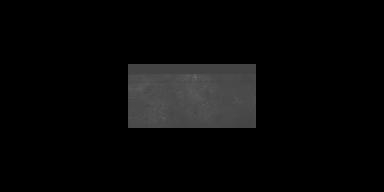
\includegraphics[width=\linewidth]{frames_1_2/frame-00001.jpg}
              \caption{Frame $1$}
          \end{figure}
      \end{minipage}
      \hspace{0.05\linewidth}
      \begin{minipage}{0.45\linewidth}
          \begin{figure}[H]
              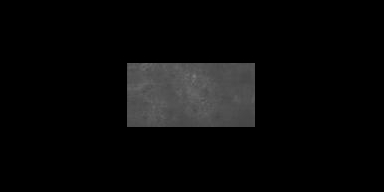
\includegraphics[width=\linewidth]{frames_1_2/frame-00002.jpg}
              \caption{Frame $2$}
          \end{figure}
      \end{minipage}
\end{minipage}
\FloatBarrier

\begin{minipage}{\linewidth}
      \centering
      \begin{minipage}{0.45\linewidth}
          \begin{figure}[H]
              \includegraphics[width=\linewidth]{frames_1_2/margin_5/lin_velocity_fitting_l1_2.jpg}
              \caption{One iteration approach, $\theta = -0.009$}
          \end{figure}
      \end{minipage}
      \hspace{0.05\linewidth}
      \begin{minipage}{0.45\linewidth}
          \begin{figure}[H]
              \includegraphics[width=\linewidth]{frames_1_2/margin_5/lin_velocity_fitting_l1_2.jpg}
              \caption{Greedy Approach, $\theta = -0.007$}
          \end{figure}
      \end{minipage}
\end{minipage}

  
\FloatBarrier
\newpage

% ------------------------------------------------------------------------------------------
\section*{Motion to the left}
% ------------------------------------------------------------------------------------------

\begin{minipage}{\linewidth}
      \centering
      \begin{minipage}{0.45\linewidth}
          \begin{figure}[H]
              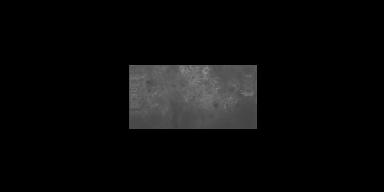
\includegraphics[width=\linewidth]{frames_47_48/frame-00047.jpg}
              \caption{Frame $1$}
          \end{figure}
      \end{minipage}
      \hspace{0.05\linewidth}
      \begin{minipage}{0.45\linewidth}
          \begin{figure}[H]
              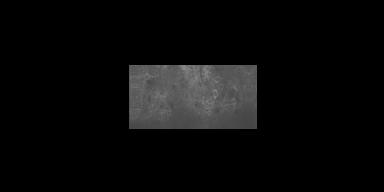
\includegraphics[width=\linewidth]{frames_47_48/frame-00048.jpg}
              \caption{Frame $2$}
          \end{figure}
      \end{minipage}
\end{minipage}
\FloatBarrier

\begin{minipage}{\linewidth}
      \centering
      \begin{minipage}{0.45\linewidth}
          \begin{figure}[H]
              \includegraphics[width=\linewidth]{frames_47_48/margin_5/lin_velocity_fitting_l1.jpg}
              \caption{One iteration approach, $\theta = -0.009$}
          \end{figure}
      \end{minipage}
      \hspace{0.05\linewidth}
      \begin{minipage}{0.45\linewidth}
          \begin{figure}[H]
              \includegraphics[width=\linewidth]{greedy_approach/frames_47_48/lin_velocity_fitting_l1.jpg}
              \caption{Greedy Approach, $\theta = -0.009$}
          \end{figure}
      \end{minipage}
\end{minipage}

  
\FloatBarrier
\newpage

% ------------------------------------------------------------------------------------------
\section*{Motion to the right}
% ------------------------------------------------------------------------------------------

\begin{minipage}{\linewidth}
      \centering
      \begin{minipage}{0.45\linewidth}
          \begin{figure}[H]
              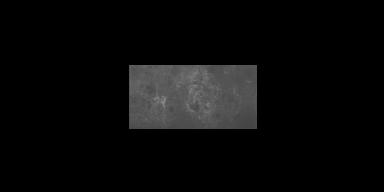
\includegraphics[width=\linewidth]{frames_84_85/frame-00084.jpg}
              \caption{Frame $1$}
          \end{figure}
      \end{minipage}
      \hspace{0.05\linewidth}
      \begin{minipage}{0.45\linewidth}
          \begin{figure}[H]
              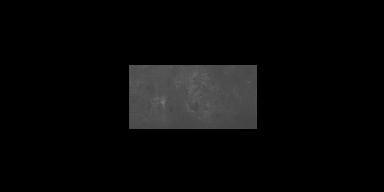
\includegraphics[width=\linewidth]{frames_84_85/frame-00085.jpg}
              \caption{Frame $2$}
          \end{figure}
      \end{minipage}
\end{minipage}
\FloatBarrier

\begin{minipage}{\linewidth}
      \centering
      \begin{minipage}{0.45\linewidth}
          \begin{figure}[H]
              \includegraphics[width=\linewidth]{frames_84_85/margin_5/lin_velocity_fitting_l1.jpg}
              \caption{One iteration approach, $\theta = 0.014$}
          \end{figure}
      \end{minipage}
      \hspace{0.05\linewidth}
      \begin{minipage}{0.45\linewidth}
          \begin{figure}[H]
              \includegraphics[width=\linewidth]{greedy_approach/frames_84_85/lin_velocity_fitting_l1.jpg}
              \caption{Greedy Approach, $\theta = 0.015$}
          \end{figure}
      \end{minipage}
\end{minipage}


\end{document}